--------------\textbf{Übungsaufgaben}--------------\\
\textbf{Zerlegung}: $Ax = (LQRDL^T)x = b$\\
\textbf{Lsg}: $Lu = b$, $Qv = u$ mit $v = Q^Tu$, $Rw = v$, $Dy = w$, $L^Tx = y$\\
-----------------------------------------------------\\
\textbf{Lsg.-Strategien}: $A \in \mathbf{R}^{21x20} \rightarrow$ QR,
da LR und Cholesky nur für quad. sinnvoll\\
$A \in \mathbf{R}^{10x10}$ sym. $\rightarrow$ Cholesky, falls spd\\
$A \in \mathbf{R}^{10x10}$ mit mind. einem Diagonaleintrag $\leq 0 \rightarrow$ LR, da A nicht pos. def.\\
$A \in \mathbf{R}^{20x21}$ (unterbestimmt) $\rightarrow$ QR von $A^T$, $R^Ty = b$ lösen (VwS), Lsg: $x = Qy$\\
-----------------------------------------------------\\
\textbf{Min-Norm}: $Rang(A) = R$, Singulärwertz. gegeben. $\mathrm{Z\kern-.6em\raise-0.7ex\hbox{Z}}$: $ x^{\dagger} = A^{\dagger}b$ ist Lsg des AGPs\\
\textbf{Lsg}: $A^TAx^{\dagger} = V \Sigma^T U^T U \Sigma V^T V \Sigma^{\dagger} U^T b = V \Sigma^T \Sigma \Sigma^{\dagger} U^T b = V \Sigma^T U^T b = A^T b$\\
\mbox{$\mathrm{Z\kern-.6em\raise-0.7ex\hbox{Z}}$: $ x^{\dagger} = \sum_{r=1}^R \frac{1}{\sigma_r}(u^r)^Tbv^r$, Lsg: $A^{\dagger}b$} $= V \Sigma^{+}U^T \sum_{m=1}^M (u^m)^T b u^m$\\
$= V \sum_{m=1}^R \frac{1}{\sigma_m} (u^m)^T b e_m$ = Ergebnis\\
-----------------------------------------------------\\
\textbf{Newton: $\frac{1}{x} - a$ ohne Div}: $x_{n+1} = x_n \\- f'(x_n)^{-1} f(x_n) = x_n - (-\frac{1}{x_n^2})^{-1}(\frac{1}{x_n} - a) = x_n(2 - ax_n)$ \textbf{Fehler}: $e_{k+1} = \frac{1}{a} - x_{k+1} = ae_k^2$\\
-----------------------------------------------------\\
\textbf{Quad. Splines} GLS ($s'_N(x_N) = v$) \textbf{Lsg}: Es gilt $s'_n(x) = y_{n-1,n} + \alpha_n(2x - x_{n-1} - x_n)$ und $s'_n(x_n) = s'_{n+1}(x_n)$ (Glattheitsbedingung) \\ 
$\Rightarrow \alpha_n h_n + \alpha_{n+1} h_{n+1} = y_{n,n + 1} - y_{n-1, n}$\\
\[\left(\begin{array}{ccc}
h_1 & h_2 & \\
 & h_{N-1} & h_N \\
 &  & h_N \\
\end{array}\right)
\left(\begin{array}{c}
\alpha_{1}\\
.\\
\alpha_{N}\\
\end{array}\right) = 
\left(\begin{array}{c}
y_{1,2} - y_{0,1}\\
.\\
v - y_{N-1,N}\\
\end{array}\right)
\]
--------------\textbf{Splines zuordnen}--------------\\
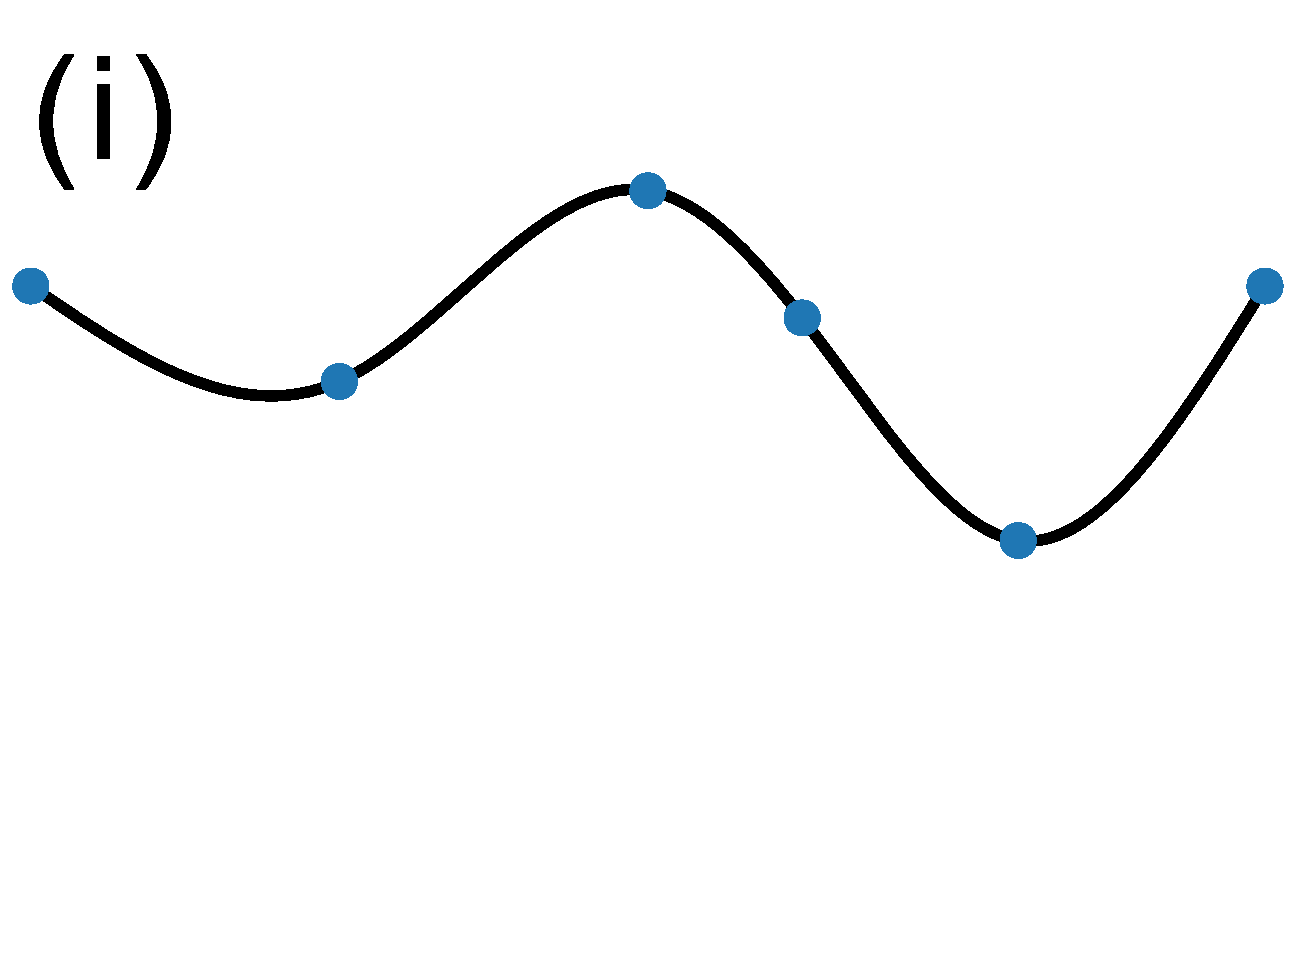
\includegraphics[scale=0.08]{content/images/spline_i.pdf}
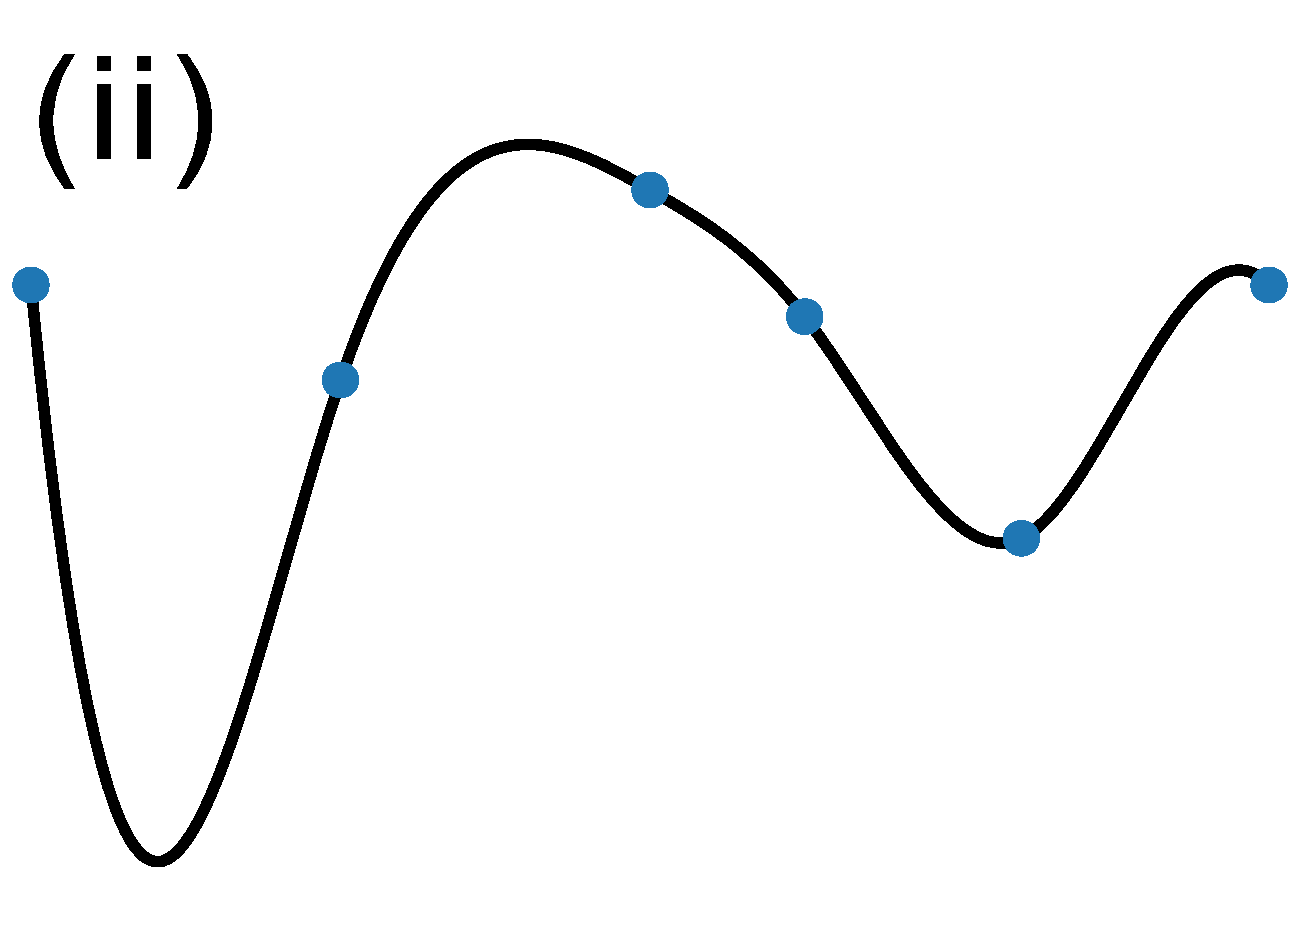
\includegraphics[scale=0.08]{content/images/spline_ii.pdf}
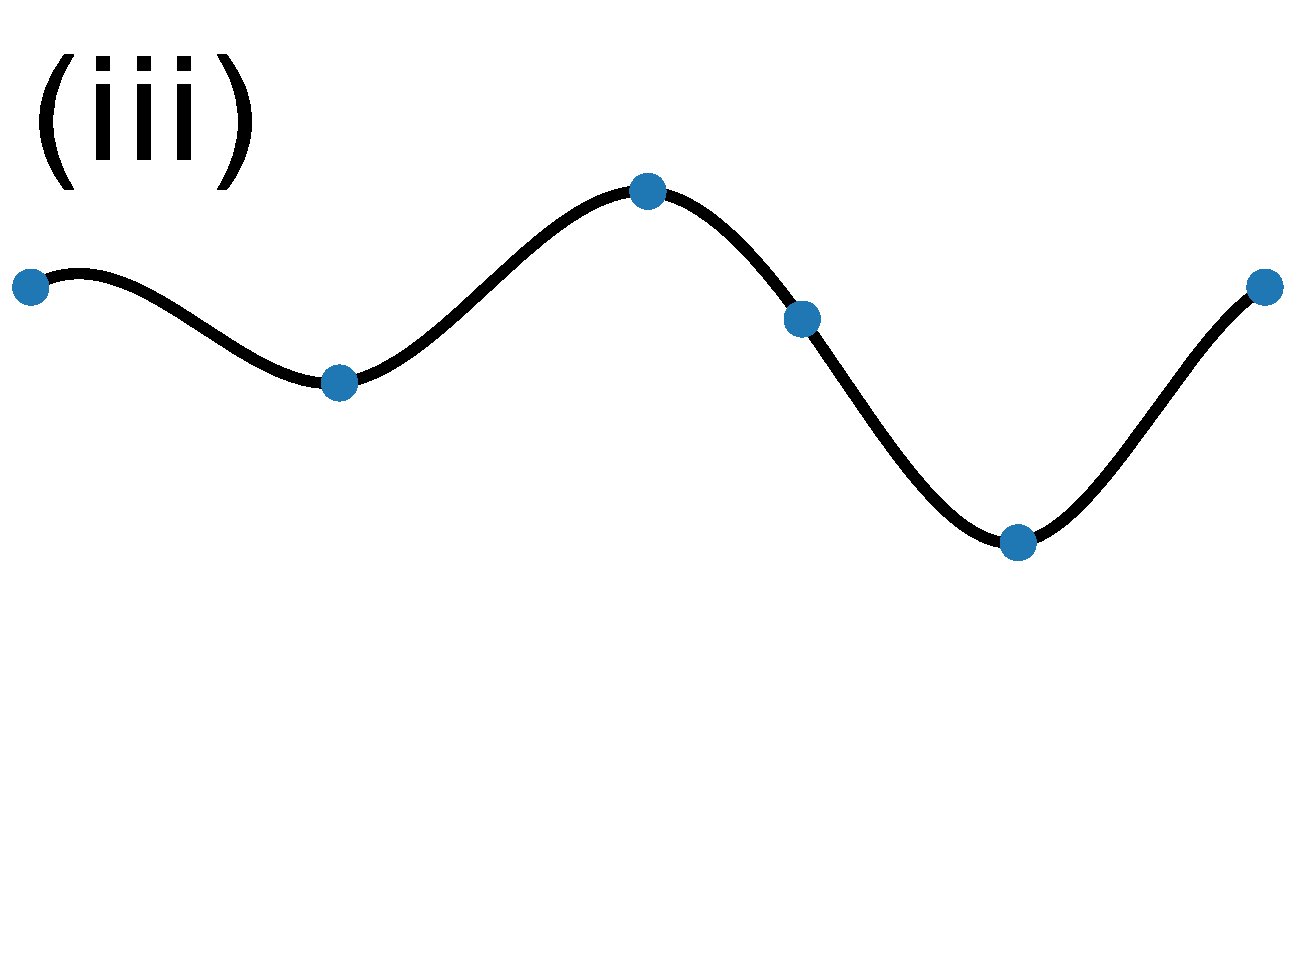
\includegraphics[scale=0.08]{content/images/spline_iii.pdf}\\
(i) natürlich, da Steigung an linken und rechtem RP $\approx$ konstant (ii) eingespannt, da nicht periodisch und nicht natürlich (iii) periodisch, da Steigung an Randpunkten $\approx$ identisch, RP: Randpunkt\\
%-----------------------------------------------------\\
-----------------------------------------------------\\
Knoten sym. $\leftrightarrow$ Ordnung p gerade. Es gilt $p \in (s, 2s]$. Da $2s$ eindeutig und Quadratur nicht identisch, gilt $p \in (s, 2s)$\\
-----------------------------------------------------\\
\textbf{Shiftmatrix}: $S = (e^N | e^1 | e^2 | ... | e^{N-1})$,\\ \hspace*{1mm}Iteration mit SV $y^0 = e^1$, konvergent?\\
\hspace*{1mm}\textbf{Lsg}: Iteration $y^{k+1} = Sy^k \rightarrow$ durchläuft \hspace*{1mm} $e^1 \rightarrow e^N \rightarrow ... \rightarrow e^1 \rightarrow$ nicht konvergent\\
-----------------------------------------------------\\
\pmb{$Q_wAQ_w$} $ = (I_k - 2ww^T)A(I_k - 2ww^T) \\= (A - 2ww^TA)(I_k -2ww^T) \\= A-2Aww^T - 2ww^TA + 4ww^TAww^T$\\
(V: $v = -2Aw$) $A + vw^T + wv^T - 2ww^Tvw^T$\\
(V: $\alpha -w^Tv$) $A + vw^T + wv^T + 2\alpha ww^T$\\
(V: $u = v + \alpha w)$ $A + uw^T + wu^T$\\
-----------------------------------------------------\\
\textbf{cg: Eigenwerte} Geg: A quad. sdp mit größtem EW $\lambda_1 > 1$ (alg. VF 1) und $|\lambda - 1| \leq \epsilon$. $\mathrm{Z\kern-.6em\raise-0.7ex\hbox{Z}}$: $||x^2 - x^*||_A \leq \epsilon||x^0 - x^*||_A$. \textbf{Lsg}: Sei $q_2(x) = \frac{1}{\lambda_1}(\lambda_1 - x)(1-x)$. Satz 39: $||x^2 - x^*|| \leq max|q_2(\lambda_j)|*||x^0 - x*||_A \\
\leq max |\frac{\lambda_1(1-\lambda_j)}{\lambda_1}|*||x^0 - x^*||_A \leq \epsilon||x^0 - x^*||_A$\\
$\mathrm{Z\kern-.6em\raise-0.7ex\hbox{Z}}$: k vers. EW $\Leftrightarrow$ exakte LSG nach k Schritten. \textbf{Lsg}: Sei $q_k(\lambda) = \prod_{j = 1}^k = \frac{\lambda_j - \lambda}{\lambda_j}$. Es gilt $q_k(0) = 1$ und $q_k(\lambda_j) = 0$. Satz 39: $||x^k - x^*||_A \leq max|q_k(\lambda_j)|*||x^0 - x^*||_A \\ = 0 \rightarrow x^k = x^*$ ist Lsg. des LGS\\
-----------------------------------------------------\\
Sei $Q_w = I_4 - 2ww^T$ die HHT mit 
$Q_wA $ \mbox{$= \{r_{11} , r_{12}^T \}, \{0_3 , A^{(1)}\}$ und A. Bestimme} \mbox{$r_{11}$. \textbf{Lsg}: $\text{Norm erster Spalte } = ||Q_wa^1||_2$} $ = ||r_{11}e^1||_2 = |r_{11}|$. Wähle VZ sodass im Zähler $a^1 - r_{11}e^1$ keine Auslöschung auftritt $\rightarrow$ Falls $a_{11}$ neg. wähle $r_{11}$ pos.\\
------ \textbf{Schritt im Newton-Verfahren} ------\\
$x \rightarrow \begin{pmatrix} x_1^2 x_2 - 1 \\ sin(x_2 \pi) \end{pmatrix}$ mit SW $x^0 = \begin{pmatrix} 0,5 \\ 2 \end{pmatrix}$. \textbf{Lsg}: $f'(x_1,x_2) = \begin{pmatrix} 2 \hspace*{3mm} 0.25\\0 \hspace*{3mm} \pi \end{pmatrix}$. Es gilt \mbox{$f'(x_1,x_2) \begin{pmatrix} d_1 \\ d_2 \end{pmatrix} = x^0$, $x = x^0 + d \rightarrow \begin{pmatrix} 0.75 \\ 2\end{pmatrix}$}\\
----------\textbf{Zusammenhang Normen}----------\
\mbox{$||x||_{\infty} = max_{1 \leq i \leq n}|x_i| = \sqrt{max_{1 \leq i \leq n}|x_i|^2}\leq$} \\
\mbox{$\sqrt{\sum_{i=1}^n|x_i|^2} = ||x||_2 \leq \sqrt{\sum_{i=1}^n} max_{1 \leq j \leq n |x_j|^2}$}\\
\mbox{$= \sqrt{n}*max_{1 \leq j \leq n}|x_j|^2 = \sqrt{n}||x||_{\infty}$}\\
-------- \textbf{Ableitungen und Sonstiges} --------\\
\mbox{$(a^x)' = (a^x) ln(a)$, \hspace{1.5mm}$\sqrt{x}' = \frac{1}{2\sqrt{x}}$, \hspace{1.5mm} GLHF :)}